\documentclass[cn,10pt,math=newtx,citestyle=gb7714-2015,bibstyle=gb7714-2015]{0-figure/en.elegantbook}

\usepackage{CJKfntef}
\usepackage{amssymb}
\usepackage{array}
\usepackage[utf8]{inputenc}
% AI说要加 \usepackage{csquotes}
%\usepackage{caption}
\usepackage{chemformula}
\usepackage{svg}
\usepackage{extarrows}
%\usepackage{0-figure/extrarelation}
\usepackage{tikz-3dplot}


\usetikzlibrary{cd}
\cover{0-figure/cover.jpg}
%%%%%%%%%%2024.10.20%%%%%%%%%
\newcommand{\ccr}[1]{\makecell{{\color{#1}\rule{1cm}{1cm}}}}

\definecolor{customcolor}{RGB}{32,178,170}
\colorlet{coverlinecolor}{customcolor}
\renewcommand{\theequation}{\thechapter.\arabic{equation}}

\usepackage{listofitems}
\newcommand\cycle[2][\,]{%
  \readlist\thecycle{#2}%
  (\foreachitem\i\in\thecycle{\ifnum\icnt=1\else#1\fi\i})%
}

\usepackage{dsfont}


\newcommand{\ve}{\varepsilon}
\DeclareMathOperator{\Int}{Int}
\DeclareMathOperator{\Ext}{Ext}
\DeclareMathOperator{\diam}{diam}


\renewcommand{\iff}{\Leftrightarrow}

\newcommand{\N}{\mathbb{N}}
\newcommand{\Z}{\mathbb{Z}}
\newcommand{\Q}{\mathbb{Q}}
\newcommand{\R}{\mathbb{R}}
\newcommand{\C}{\mathbb{C}}
\newcommand{\FF}{\mathbb{F}}
\newcommand{\RP}{\mathbb{R}\mathbb{P}}
\newcommand{\CP}{\mathbb{C}\mathbb{P}}
\renewcommand{\P}{\mathcal{P}}


\newcommand{\z}{\left}
\newcommand{\y}{\right}

\newcommand{\letgroup}{令$(G,\cdot)$是一个群}
\newcommand{\letaction}{令$\phi:(G,\cdot)\to (\perm(S),\circ)$是一个$G$在$S$的群作用}
\DeclareMathOperator{\ima}{im}
\DeclareMathOperator{\perm}{Perm}
\DeclareMathOperator{\orb}{Orb}
\DeclareMathOperator{\stab}{Stab}


\newcommand{\letring}{令$(R,+,\cdot)$是一个环}
\newcommand{\letcommring}{令$(R,+,\cdot)$是一个交换环}
\newcommand{\letintdom}{令$(R,+,\cdot)$是一个整环}
\newcommand{\letpid}{令$(R,+,\cdot)$是一个主理想整环}
\newcommand{\letufd}{令$(R,+,\cdot)$是一个唯一分解整环}
\newcommand{\letucd}{令$(R,+,\cdot)$是一个最大公因数整环}
\newcommand{\leted}{令$(R,+,\cdot)$是一个欧几里得整环}
\newcommand{\letfield}{令$(F,+,\cdot)$是一个域}
\DeclareMathOperator{\lcm}{lcm}
\DeclareMathOperator{\cont}{cont}
%\DeclareMathOperator{\ch}{char}
\newcommand{\letext}{令$F/E$是一个域扩张}

\newcommand{\lethomring}{令$f:(R,+,\cdot)\to (R',+,\cdot)$是一个环同态}
\newcommand{\p}{\mathfrak{p}}
\newcommand{\m}{\mathfrak{m}}


\newcommand{\sss}{\sum_{i=1}^{n}}
\DeclareMathOperator{\F}{Frac}

\DeclareMathOperator{\spn}{span}


\DeclareMathOperator{\Hom}{Hom}
\DeclareMathOperator{\A}{\mathds{A}}\DeclareMathOperator{\G}{Gal}
\DeclareMathOperator{\Tr}{Tr}
\renewcommand{\O}{\mathcal{O}}

\DeclareMathOperator{\del}{\partial}

\newcommand{\ii}{\int^b_a}
\newcommand{\ff}{f^{-1}}
\newcommand{\Lim}{\lim\limits_{x\to 0}}
\renewcommand{\epsilon}{\varepsilon}
\renewcommand{\implies}{\Rightarrow}
\renewcommand{\impliedby}{\Leftarrow}
\newcommand{\dx}{\ \mathrm{d}x}
\newcommand{\dt}{\ \mathrm{d}t}
\newcommand{\du}{\ \mathrm{d}u}
\newcommand{\dz}{\ \mathrm{d}z}
\newcommand{\dy}{\ \mathrm{d}y}
\newcommand{\df}{\ \mathrm{d}f}

\title{Calculus Handout}
\author{Chharlie1130}
\date{\today}

\begin{document}
\maketitle
\frontmatter

\newpage

\tableofcontents
\mainmatter


\chapter*{Preface}
\addcontentsline{toc}{chapter}{Preface}
\markboth{Preface}{}%I don't know why, but the author says so: to let me put empty brackets here.

\section{Is This Handout for You?}
This handout is created to help students understand calculus with stress on computation techniques rather than rigorous proofs. The goal is to present the material clearly and organized, making it easier to follow and apply in practical problems.


The main focus will be on solving problems effectively using methods from differentiation and integration rather than delving into the theoretical foundations of calculus. 
\section{What's in This Handout?}

Throughout this handout, I have reorganized the content in a way that I believe will help students learn the topics more logically. The sequence is designed to build from basic concepts to more complex ones, allowing for a smoother learning experience.


The abstract of this course is mentioned below, which will serve as
a roadmap for you to gain the essence of calculus.
\begin{introduction}[Core concept]
    \item Limits and Continuity
    \item Derivatives
    \item Integrals
    \item Series
\end{introduction}

\section{How to Read this Handout?}
\begin{itemize}
    \item Do examine the given conditions carefully! Mostly, they are as important as the conclusion of a theorem.
    \item Refer the other books if you find some of the content looks hard to understand. (This is also practical when you are reading any other math books)
\end{itemize}




I hope this handout serves as a helpful guide for students looking to strengthen their calculation abilities and build a strong foundation in calculus.

\chapter{Prerequisite}

\section{Important Things in a Math Book}

\chapter{Limits and Continuity}

\section{Limit of a Function}

\section{Limit of a Sequence}
\subsection{Convergence and Divergence}

\section{Limit Laws of Function and Sequence}
\subsection{Limit Laws of Function}
\subsection{Limit Laws of Sequence}
\subsection{The Sandwich Theorem}
\subsection{An Important Limit}

\section{Continuity}
\subsection{}

\chapter{Derivatives}
\section{Big-O and Little-o Notation}
\textbf{Big-O Notation}, along with \textbf{Little-o Notation}, tell you how fast a function grows and declines.
Obviously, this notation is abusing the equality symbol, since it violates the axiom of
equality: "things equal to the same thing are equal to each other"
. To be more formally
correct, some people (mostly mathematicians, as opposed to computer scientists) prefer
to define O(g(x)) as a set-valued function, whose value is all functions that do not grow
faster then g(x), and use set membership notation to indicate that a specific function is a
member of the set thus defined. Both forms are in common use, but the sloppier equality
notation is more common at present.

\chapter{Applications of Derivatives}
\section{Motivation}
% Creating logic sequence with arrows for theorems
\[
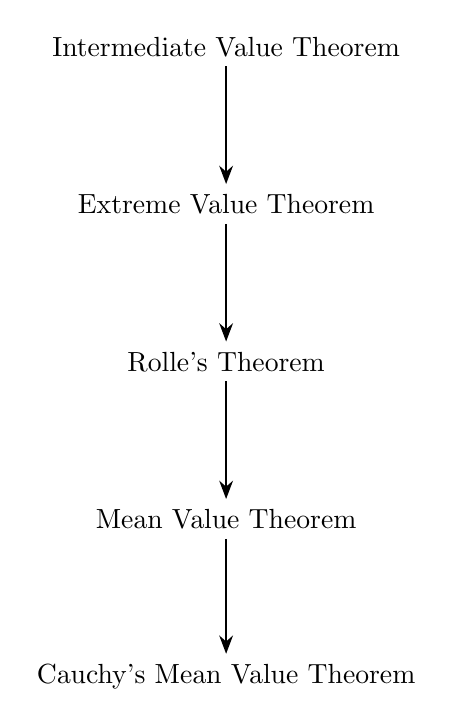
\begin{tikzpicture}[>=Stealth, thick]
    % Intermediate Value Theorem
    \node (IVT) at (0, 0) {Intermediate Value Theorem};
    % Extreme Value Theorem
    \node (EVT) at (0, -2) {Extreme Value Theorem};
    % Rolle's Theorem
    \node (RT) at (0, -4) {Rolle's Theorem};
    % Mean Value Theorem
    \node (MVT) at (0, -6) {Mean Value Theorem};
    % Cauchy's Mean Value Theorem
    \node (CMVT) at (0, -8) {Cauchy's Mean Value Theorem};
    
    % Arrows showing implication
    \draw[->] (IVT) -- (EVT);
    \draw[->] (EVT) -- (RT);
    \draw[->] (RT) -- (MVT);
    \draw[->] (MVT) -- (CMVT);
\end{tikzpicture}
\]


\section{Theorems and Tools for Analyzing Function Extremes}
\subsection{Intermediate Value Theorem}
\subsection{Extreme Value Theorem}
\subsection{Rolle's Theorem}
\subsection{Mean Value Theorem}

\section{Indeterminate Forms and L'Hôpital's Rule}
\subsection{Cauchy's Mean Value Theorem}
\subsection{Indeterminate Form $0/0$}
\subsection{L'Hôpital's Rule}

\chapter{Integrals}
\section{Motivation}
\subsection{Definite and Indefinite Integrals}

\section{Antiderivatives}

\section{Riemann Sums}


\section{The Fundamental Theorem of Calculus}

\chapter{Techniques of Integration}
\section{Substitution}


\section{Integration by Parts}



\section{Partial Fractions}

\chapter{Applications of Definite Integrals}

\chapter{}




%\printbibliography
\end{document}
